\begin{abstract}
    In this paper, I present the background, theory, and design considerations for a resonant filter which implements voltage control by use of a diode ladder. The theoretical background to understand resonance and voltage control are explored, and experimentally determined configurations are presented which optimize performance characteristics suitable for audio synthesis applications.
\end{abstract}

\section{Introduction}\label{sec:introduction}

Active filters are an essential and classic ingredient in an audio engineer's toolkit. The walls of knobs and dials commonly associated with synthesizers and studios are really some massive array of such devices which may be tuned by an artist to produce some of our favorite sounds in music. Audio engineering is one of the realms in which such analog devices still flourish in tandem with digital equipment, and in this project I aim to explore the mechanisms of voltage-controlled amplification and resonance in one such active filter.

Throughout this course, we have dealt with amplification and impedance matching via op-amps. This a key element in basic resonant filter design, allowing us to maintain control over cutoff and create a circuit which can operate in a huge range of input signal types. I incorporate seven op-amp devices in this circuit, which will be discussed further in the following sections.

The mechanism by which a signal is shaped to have a particular sound is through the addition of resonance to a waveform. Non-resonant filters can be thought of as a precise and controlled filter, typically strongly cutting off an output frequency or voltage after a certain point. Resonant filters, on the other hand are capable of emphasizing certain frequencies near the cutoff point, an example of which is shown in Figure \ref{fig:resonance}. It is through the emphasis of certain frequencies this mechanism that an input signal can be shaped to have a sound quality, from a bass to a drum.

We describe the operation of a resonant filter by the overshooting and undershooting phases introduced, in this case by op-amps. As resonance is raised, it appears as though the filter takes longer to settle on its frequency, much like a damped oscillator which we are controlling the damping rate. Furthermore, as cutoff is lowered, the waveform additionally remains in over and undershooting phases for longer, akin to adjusting the mass of a damped oscillator. Such behavior can be seen in Figure \ref{fig:resonance}.

\subsection{Basic Resonant Filters}

The simplest resonant filter, shown in Figure \ref{fig:simple-filter} operates on the principle of negative feedback introduced by a combination of followers and capacitors. Consider the input to be a square wave rising from 0 to 5 volts. At the instant the signal goes high, the first capacitor fills and follower begins to raise the voltage at its output to match the non-inverting input signal, soon after filling the second capacitor and raising the voltage after the second follower. Something unusual happens now, and because of the first capacitor the voltage going into the first follower continues to rise past 5 V. Because of the first resistor, the resistor acts like an equalizing valve, dissipating some of this additional charge on the capacitor after some time, bringing the voltage back down, below 5 V. At this point, the first capacitor is not fully empty, repeating the overshooting phase with a smaller peak, which causes an undershooting phase afterwards. This cycle repeats again and again until after some time the circuit stabilizes at 5 V. 

\begin{figure}[H]
    \par\noindent\rule{\textwidth}{0.4pt} \vspace{4em}
    \centering
    \begin{subfigure}[b]{1\textwidth}
        \vspace{2em}
        \captionsetup{labelformat=empty}
        \begin{picture}(0,0)
            \put(-10,90){\small\textbf{(a)}}
        \end{picture}
        \centering
        \resizebox{0.85\textwidth}{!}{%
            \begin{circuitikz}
                \tikzstyle{every node}=[font=\LARGE]
                \draw (8.25,16) node[op amp,scale=1, yscale=-1 ] (opamp2) {};
                \draw (opamp2.+) to[short] (6.75,16.5);
                \draw  (opamp2.-) to[short] (6.75,15.5);
                \draw (9.45,16) to[short](9.75,16);
                \draw (0.75,16) to[short, -o] (-0.25,16) node[above] {In};
                \draw (1.75,16) to[R,l={ \LARGE 100 k$\Omega$}] (3.5,16);
                \draw (4,16) to[short] (4,14.5);
                \draw (4,13.75) to[C,l={ \LARGE 10 nF}] (4,13);
                \draw (6.75,15.5) to[short] (6.75,14.5);
                \draw (6.75,14.5) to[short] (9.75,14.5);
                \draw (9.75,14.5) to[short] (9.75,16);
                \draw (9.75,16) to[R,l={ \LARGE 100 k$\Omega$}] (12.25,16);
                \node at (4,16) [circ] {};
                \draw (12.25,16) to[short] (12.25,14);
                \draw (12.25,14) to[C,l={ \LARGE 10 nF}] (12.25,13.25);
                \draw (12.25,13.25) to (12.25,13) node[ground]{};
                \draw (5.75,16) to[short] (5.75,16.5);
                \draw (5.75,16.5) to[short] (6.75,16.5);
                \draw (18,14.5) to[short] (18,16);
                \draw (16.5,16) node[op amp,scale=1, yscale=-1 ] (opamp2) {};
                \draw (opamp2.+) to[short] (15,16.5);
                \draw  (opamp2.-) to[short] (15,15.5);
                \draw (17.7,16) to[short](18,16);
                \draw (15,14.5) to[short] (18,14.5);
                \draw (14,16) to[short] (14,16.5);
                \draw (14,16.5) to[short] (15,16.5);
                \draw (13.5,16) to[short] (14,16);
                \draw (12.75,16) to[short] (13.5,16);
                \draw (3.5,16) to[short] (4,16);
                \draw (4,16) to[short] (5.75,16);
                \draw (12.25,16) to[short] (12.75,16);
                \draw (15,14.5) to[short] (15,15.5);
                \draw (19.75,16) to[short] (19.75,11.5);
                \draw (4,11.5) to[short] (19.75,11.5);
                \draw (19.75,16) to[short, -o] (21.75,16) node[above] {Out};
                \draw (19.75,16) to[short] (18,16);
                \draw (4,11.5) to[short] (4,13);
                \draw (4,13.75) to[short] (4,14.5);
                \draw (0.75,16) to[short] (1.75,16);
                \node at (12.25,16) [circ] {};
                \node at (19.75,16) [circ] {};
                \node at (18,16) [circ] {};
                \node at (9.75,16) [circ] {};
            \end{circuitikz}
            }
            \caption{}
            \label{fig:simple-filter}
    \end{subfigure}
    % Second subfigure: Output image
    \begin{subfigure}[b]{0.85\textwidth}
        \vspace{-3em}
        \captionsetup{labelformat=empty}
        \begin{picture}(0,0)
            \put(-10,20){\small\textbf{(b)}}
        \end{picture}
        \includegraphics[width=\textwidth,valign=t]{../assets/simple-filter-output.png}
        \caption{}
        \label{fig:simple-filter-output}
    \end{subfigure}

    \caption{\textbf{(a)} Simple resonant filter driven by a combination of capacitors, resistors, and op-amps. As the waveform goes high at the input, the capacitor is filled and the first op-amp, in follower configuration, begins to raise the voltage. Due to the resistor, current flows backwards, causing the output of the first op-amp to overshoot and form the first crest of the resonant output. The capacitor then discharges and the follower "catches up" and begins lowering the output voltage. Again, this overshoots, and we reach the bottom of the first valley. The capacitor is still partially filled, and will begin to overshoot once more, reaching a lower peak than before. This cycle repeats until the signal goes low. \textbf{(b)} The input (left) and output (right) signals, simulated using falstad.} 
    \label{fig:combined-filter}
    \par\noindent\rule{\textwidth}{0.4pt}
\end{figure}


\subsection{Fully Resonant Filters}\label{sec:fully-resonant-LPF}

This is great, but we have no control over this circuit without directly replacing components. We can fix this by introducing a potentiometer to vary the resistance at the bottom line of Figure \ref{fig:simple-filter}. This is fed through an op amp configured to provide a stable current. This circuit is susceptible to clipping as the cutoff is raised as the output can easily exceed the 12 V maximum of the TL074 OP-Amps, so I add a 10\% voltage divider and AC Coupling with a follower to stabilize current at the input. This is an improvement over the basic resonant filter, however we still lack key features of cutoff control that is necessary for a voltage controlled filter.

\begin{figure}[H]
    \par\noindent\rule{\textwidth}{0.4pt} \vspace{4em}
    \centering
    \resizebox{1\textwidth}{!}{%
        \begin{circuitikz}
            \tikzstyle{every node}=[font=\Large]
            \draw (8.25,16) node[op amp,scale=1, yscale=-1] (opamp1) {};
            \draw (opamp1.+) to[short] (6.75,16.5);
            \draw (opamp1.-) to[short] (6.75,15.5);
            \draw (opamp1.out) to[short] (9.75,16);
            \draw (1.75,16) to[R,l=$100~\text{k}\Omega$] (3.5,16);
            \draw (6.75,15.5) to[short] (6.75,14.5);
            \draw (6.75,14.5) to[short] (9.75,14.5);
            \draw (9.75,14.5) to[short] (9.75,16);
            \node at (4,16) [circ] {};
            \draw (12.25,16) to[short] (12.25,15);
            \draw (12.25,15) to[C,l=$10~\text{nF}$] (12.25,14.25);
            \draw (5.75,16) to[short] (5.75,16.5);
            \draw (5.75,16.5) to[short] (6.75,16.5);
            \draw (3.5,16) to[short] (4,16);
            \draw (4,16) to[short] (5.75,16);
            \draw (0.75,16) to[short] (1.75,16);
            \node at (12.25,16) [circ] {};
            \node at (9.75,16) [circ] {};
            \draw (0.75,16) to[C,l=$1~\mu\text{F}$] (-1.25,16);
            \draw (-1.25,16) to[short, -o] (-2,16) node[above] {In};
            \draw (0.75,16) to[R,l=$200~\text{k}\Omega$] (0.75,13.5);
            \draw (0.75,13.5) to (0.75,13) node[ground]{};
            \draw (4,16) to[R,l=$33~\text{k}\Omega$] (4,13.5);
            \draw (4,13.5) to (4,13) node[ground]{};
            \draw (9.75,16) to[potentiometer,l=$100~\text{k}\Omega$] (12.25,16);
            \draw (14.5,11.75) node[op amp,scale=1, xscale=-1, yscale=-1] (opamp2) {};
            \draw (opamp2.+) to[short] (16,12.25);
            \draw (opamp2.-) to[short] (16,11.25);
            \draw (opamp2.out) to[short] (13,11.75);
            \draw (13.5,9) to[R,l=$10~\text{k}\Omega$] (15.5,9);
            \draw (13,11.75) to[short] (13,9);
            \draw (16,11.25) to[short] (16,9);
            \draw (16,9) to[short] (15.5,9);
            \draw (13,9) to[short] (13.5,9);
            \draw (13,11.75) to[short] (12.25,11.75);
            \draw (12.25,11.75) to[short] (12.25,14.25);
            \draw (15.5,9) to[R,l=$60~\text{k}\Omega$] (15.5,6.25);
            \draw (15.5,6.25) to (15.5,5.75) node[ground]{};
            \draw (16.5,16) node[op amp,scale=1, yscale=-1] (opamp3) {};
            \draw (opamp3.+) to[short] (15,16.5);
            \draw (opamp3.-) to[short] (15,15.5);
            \draw (opamp3.out) to[short] (18,16);
            \draw (15,15.5) to[short] (15,14.5);
            \draw (15,14.5) to[short] (18,14.5);
            \draw (14,16) to[short] (14,16.5);
            \draw (14,16.5) to[short] (15,16.5);
            \draw (12.25,16) to[short] (14,16);
            \draw (18,14.5) to[short] (18,16);
            \draw (18,16) to[potentiometer,l=$100~\text{k}\Omega$] (20.5,16);
            \draw (20.5,16) to[C,l=$10~\text{nF}$] (20.5,13.5);
            \draw (20.5,13.5) to (20.5,13.25) node[ground]{};
            \draw (24.75,16) node[op amp,scale=1, yscale=-1] (opamp4) {};
            \draw (opamp4.+) to[short] (23.25,16.5);
            \draw (opamp4.-) to[short] (23.25,15.5);
            \draw (opamp4.out) to[short] (26.25,16);
            \draw (23.25,15.5) to[short] (23.25,14.5);
            \draw (23.25,14.5) to[short] (26.25,14.5);
            \draw (22.25,16) to[short] (22.25,16.5);
            \draw (22.25,16.5) to[short] (23.25,16.5);
            \draw (20.5,16) to[short] (22.25,16);
            \draw (26.25,14.5) to[short] (26.25,16);
            \draw (26.25,16) to[short] (27.25,16);
            \draw (27.25,16) to[short] (27.25,13.5);
            %\draw (27.25,11) to[potentiometer,l=$100~\text{k}\Omega$] (27.25,13.5);
            \draw (27.25,11) to[potentiometer,] (27.25,13.5);
            \draw (16,12.25) to[short] (26.75,12.25);
            \draw (27.25,11) to (27.25,10) node[ground]{};
            \draw (27.25,16) to[C,l=$1~\mu\text{F}$] (28.5,16);
            \draw (28.5,16) to[R,l=$200~\text{k}\Omega$] (28.5,14.25);
            \draw (28.5,14.25) to (28.5,13.75) node[ground]{};
            \draw (28.5,16) to[short, -o] (30.5,16) node[above] {Out};
        \end{circuitikz}
        }%
        \vspace{-3em}
        \caption{A diagram of a fully resonant LPF. Two adjustments are made from the basic resonant filter: (1) a potentiometer and op-amp in amplifier configuration are added after the first capacitor to allow adjustment of potential on this line, allowing operators to adjust resonance intensity, or how "high" the oscillations get. (2) A sequence of AC coupling and a 25\% voltage divider fed through a follower are added to the input line to scale down the input to avoid clipping.}
        \label{fig:fully-resonant-LPF}
        \par\noindent\rule{\textwidth}{0.4pt}
    \end{figure}


\subsection{Diodes as Voltage Controlled Resistors}\label{sec:diode-resistor}

One way to achieve cutoff control is via diodes. From this course, it is well understood that diodes have a fixed drop. This is a useful fact, as this gives a different perceived resistance of the component depending on the voltage it receives. See Figure \ref{fig:voltage-resistor} for a demonstration of this effect.

\begin{figure}[H]
    \centering
    \par\noindent\rule{\textwidth}{0.4pt} \vspace{4em}
    \hfill\hspace{1em}
    \begin{subfigure}[b]{0.22\textwidth}
        \vspace{1em}
        \centering
        \resizebox{\textwidth}{!}{%
            \begin{circuitikz}
                \tikzstyle{every node}=[font=\large]
                \draw (13.75,14.5) to[R,l={ \large 200 k$\Omega$}] (13.75,11.5);
                \draw (11.25,14.5) to[D] (11.25,11.5);
                \draw (11.25,11.5) to (11.25,11.25) node[ground]{};
                \draw (13.75,11.5) to (13.75,11.25) node[ground]{};
                \draw (11.25,14.5) to[short] (13.75,14.5);
                \draw (12.5,14.5) to[short, -o] (12.5,15.75) node[above] {300 mV};
                \node at (12.5,14.5) [circ] {};
                \node [font=\large] at (12.5,12.5) {1.5 $\mu A$};
                \draw [dashed] (12.5,14) -- (12.5,13);
                \draw [->, >=Stealth, dashed] (12.5,12) -- (12.5,11);
            \end{circuitikz}
            }
            %\caption{R = 200 k$\Omega$}
    \end{subfigure}
    \hfill
    \begin{subfigure}[b]{0.22\textwidth}
        \vspace{1em}
        \centering
        \resizebox{\textwidth}{!}{%
            \begin{circuitikz}
                \tikzstyle{every node}=[font=\large]
                \draw (13.75,14.5) to[R,l={ \large 1 k$\Omega$}] (13.75,11.5);
                \draw (11.25,14.5) to[D] (11.25,11.5);
                \draw (11.25,11.5) to (11.25,11.25) node[ground]{};
                \draw (13.75,11.5) to (13.75,11.25) node[ground]{};
                \draw (11.25,14.5) to[short] (13.75,14.5);
                \draw (12.5,14.5) to[short, -o] (12.5,15.75) node[above] {600 mV};
                \node at (12.5,14.5) [circ] {};
                \node [font=\large] at (12.5,12.5) {580 $\mu A$};
                \draw [dashed] (12.5,14) -- (12.5,13);
                \draw [->, >=Stealth, dashed] (12.5,12) -- (12.5,11);
            \end{circuitikz}
            }
            %\caption{R = 1 k$\Omega$}
    \end{subfigure}
    \hfill
    \begin{subfigure}[b]{0.22\textwidth}
        \vspace{1em}
        \centering
        \resizebox{\textwidth}{!}{%
            \begin{circuitikz}
                \tikzstyle{every node}=[font=\large]
                \draw (13.75,14.5) to[R,l={ \large 5 k$\Omega$}] (13.75,11.5);
                \draw (11.25,14.5) to[D] (11.25,11.5);
                \draw (11.25,11.5) to (11.25,11.25) node[ground]{};
                \draw (13.75,11.5) to (13.75,11.25) node[ground]{};
                \draw (11.25,14.5) to[short] (13.75,14.5);
                \draw (12.5,14.5) to[short, -o] (12.5,15.75) node[above] {500 mV};
                \node at (12.5,14.5) [circ] {};
                \node [font=\large] at (12.5,12.5) {90 $\mu A$};
                \draw [dashed] (12.5,14) -- (12.5,13);
                \draw [->, >=Stealth, dashed] (12.5,12) -- (12.5,11);
            \end{circuitikz}
            }
            %\caption{R = 5 k$\Omega$}
    \end{subfigure}
    \hfill\hspace{1em}

    \vspace{-3em}
    \caption{\textbf{(a)} A diode receiving 300 mV at its input drops by a constant voltage so we see 1.5 $\mu A$ across which is analagous to a 200 k$\Omega$ resistor. \textbf{(b)} If a diode instead receives 600 mV and we see 580 $\mu A$ across, analagous to 1 k$\Omega$. \textbf{(c)} Again, if we apply 500 mV and get a 90 $\mu A$ current, this is analagous to a 5 k$\Omega$ resistor. It appears as though the input voltage controls the output voltage.}
    \label{fig:voltage-resistor}
    \par\noindent\rule{\textwidth}{0.4pt}
\end{figure}


\subsection{Multi-Pole Diode Ladder}\label{sec:diode-ladder}

To apply this principle, we integrate diodes in a ladder, shown in Figure \ref{fig:multi-pole-diode-ladder}. This creates a copy of our input signal at some high and low offset, shown in figure \ref{fig:square-waves-annotated}, from which we can take at the center of the ladder to the output stage. Modulation of the separation difference allows us to modulate cutoff.

A degree of control we may engineer here is the number of poles of the ladder, which is qualitatively responsible for the sound quality coming out of the instrument. 5 are chosen in this instance, but adding more will further increase the separation, and fewer decrease it. Too few or too many may limit the functionality of the instrument as clipping can be a concern depending on resonance.

%\begin{figure}[!ht]
%    \centering
%
%    % First subfigure: Circuit diagram
%    \begin{subfigure}[b]{0.45\textwidth}
%    \centering
%    \resizebox{\textwidth}{!}{%
%    \begin{circuitikz}
%    \tikzstyle{every node}=[font=\LARGE]
%    \draw (2.25,15.5) to[D] (2.25,14.25);
%    \draw (2.25,14.25) to[D] (2.25,13);
%    \draw (2.25,13.25) to[D] (2.25,12);
%    \draw (2.25,12) to[D] (2.25,10.75);
%    \draw (2.25,10.75) to[D] (2.25,9.5);
%    \draw (2.25,9.5) to[D] (2.25,8.25);
%    \draw (2.25,7.75) to[short] (2.25,8.5);
%    \draw (2.25,15.5) to[short] (2.25,16);
%    \draw (2.25,14.25) to[C] (0,14.25);
%    \draw (2.25,13.25) to[C] (0,13.25);
%    \draw (2.25,12) to[C] (0,12);
%    \draw (2.25,10.75) to[C] (0,10.75);
%    \draw (2.25,9.5) to[C] (0,9.5);
%    \draw (0,10.75) to (-0.25,10.75) node[ground]{};
%    \draw (0,12) to (-0.25,12) node[ground]{};
%    \draw (0,13.25) to (-0.25,13.25) node[ground]{};
%    \node at (2.25,9.75) [circ] {};
%    \node at (2.25,10.75) [circ] {};
%    \node at (2.25,12) [circ] {};
%    \node at (2.25,13.25) [circ] {};
%    \end{circuitikz}
%    }
%    \caption{Centered schematic}
%    \label{fig:circuit_schematic}
%    \end{subfigure}
%    \hfill
%     %Second subfigure: Image
%    %\begin{subfigure}[b]{0.45\textwidth}
%    %\centering
%    %\includegraphics[width=\textwidth]{../../assets/square_waves.png}
%    %\caption{Annotated Square Waves}
%    %\label{fig:square-waves}
%    %\end{subfigure}
%
%    \caption{Overview of the circuit and signal behavior}
%    \label{fig:combined_figure}
%\end{figure}

\begin{figure}[H]
    \par\noindent\rule{\textwidth}{0.4pt} \vspace{3em}
    \hspace{2em} 
    \begin{subfigure}[b]{0.2\textwidth}
        \vspace{3em}
        \centering
        \captionsetup{labelformat=empty}
        \begin{picture}(0,0)
            \put(-55,-10){\small\textbf{(a)}}
        \end{picture}
        \includegraphics[width=\textwidth,valign=t]{../../assets/multi_pole_diode_ladder.png}
        \caption{}
        \label{fig:multi-pole-diode-ladder}
    \end{subfigure}
    \hfill
    \begin{subfigure}[b]{0.45\textwidth}
        \captionsetup{labelformat=empty}
        \begin{picture}(0,0)
            \put(0,20){\small\textbf{(b)}}
        \end{picture}
        \includegraphics[width=\textwidth,valign=t]{../../assets/square_waves_annotated.png}
        \vspace{0.5cm}
        \caption{}
        \label{fig:square-waves-annotated}
    \end{subfigure}
    \hspace{2em} 
    \vspace{-3em}
    \caption{\textbf{(a)} A sub-schematic of the diode ladder. a high and low signal copy are passed into the beginning and end of the ladder, respectively. Output is taken from the middlemost pole and fed through to produce resonance. The output of the amplification stage is then fed back into the diode ladder through the capacitors on the left. \textbf{(b)} Signals seen by different poles of the diode ladder. Separation is voltage controlled due to the mechanism discussed in Section 1.3.}
    \label{fig:diode-ladder-bits}
    \par\noindent\rule{\textwidth}{0.4pt}
\end{figure}


\subsection{Input Stage}\label{sec:input-stage}

To drive this diode ladder, one might imagine they wish to produce some DC offset which can be added or subtracted from the input waveform. This is a simple application of an inverter and adder; however, it would benefit us to use fewer op-amps as this sequence of operation could be simplified. Furthermore, we must also maintain the small oscillation size and clipping control implemented in Section \ref{sec:fully-resonant-LPF}. This prompts us to implement a new driver, shown in Figure \ref{fig:ladder-input-stage}.

\begin{figure}[H]
    \par\noindent\rule{\textwidth}{0.4pt}
    \centering
    \includegraphics[width=0.8\textwidth]{../../assets/input_stage.png}
    \caption{Input stage, handling input signal, subtracting and adding the cutoff value, and feeding this into the diode ladder's first and last poles. The input (top left) is adapted from the fully resonant filter, wherein a signal is AC coupled, passes through a 10\% voltage divider, and follower to stabilize current. The cutoff control (bottom left) implements two control methods: potentiometer and voltage control. This passes through a 0.2\% voltage divider and an additional resistor before encountering a string of three diodes. These are implemented to avoid large bias at the non-inverting input, as it is experimentally determined that voltages exceeding 1.4 V introduce clipping at the diode ladder.}
    \label{fig:ladder-input-stage}
    \par\noindent\rule{\textwidth}{0.4pt}
\end{figure}


%It's clear several aspects of these simple designs make it into the design which is built in this project, shown in Figure \ref{fig:ladder-filter}; namely, the input stage is identical, only with adjustments in resistance. It may seem different, but the negative-feedback driver for resonance shown in Figure \ref{fig:fully-resonant-LPF} makes its way into this design as well, only with the addition of some diodes to linearise the exponential response.

\subsection{Resonance}\label{sec:resonance}

Resonance in the circuit is introduced in the same fashion of Section \ref{sec:fully-resonant-LPF} by means of routing the output from the diode ladder through a follower and potentiometer through an amplifying op-amp back into the filter's upper AND lower points to preserve symmetry. Additional diodes are added to the amplifying op-amp to introduce a necessary non-linearity in its operation. Ordinarily, an op-amp in a multiplying configuration produce a constant gain which will quickly overpower the bias current and cause the diode ladder to shut down. Using the same principles as in Section \ref{sec:diode-resistor}, we know that diodes act as exponential resistors in response to voltage, and implementing them in this fashion gives an exponentially decaying gain. A comparison is available in Figure \ref{fig:gains}

\begin{figure}[H]
    \par\noindent\rule{\textwidth}{0.4pt}
    \centering
    \hspace{1em} 
    \begin{subfigure}{0.3\textwidth}
        \vspace{2em}
        \captionsetup{labelformat=empty}
        \begin{picture}(0,0)
            \put(0,-5){\small\textbf{(a)}}
        \end{picture}
        \includegraphics[width=\textwidth,valign=t]{../../assets/resonance.png}
        \caption{}
        \label{fig:resonance}
    \end{subfigure}
    \hfill
    \begin{subfigure}{0.65\textwidth}
        \captionsetup{labelformat=empty}
        \begin{picture}(0,0)
            \put(0,15){\small\textbf{(b)}}
        \end{picture}
        \includegraphics[width=\textwidth,valign=t]{../../assets/gains.pdf}
        \caption{}
        \label{fig:gains}
    \end{subfigure}
    \caption{\textbf{(a)} A sub-schematic of the op-amp configurations responsible for resonance. The amplifier outputs to the diode ladder's beginning and end poles. Output is taken from the center pole of the ladder and fed through a potentiometer to the non-inverting input, producing resonance. \textbf{(b)} Demonstration of the effect on output from introducing diodes on the amplifier. Data is simulated in LTSpice, where an approximately constant gain (or linear output voltage) is produced when there are no diodes in the circuit. By introducing diodes, there is exponential loss in gain (or exponential decay in output voltage).}
    \label{fig:combined}
    \par\noindent\rule{\textwidth}{0.4pt}
\end{figure}


\section{Experimental Technique}

\subsection{Fabrication}
Our voltage-controlled, diode ladder-based resonant filter is implemented on breadboard, shown in Figure \ref{fig:breadboard}. The components used are listed in Figure \ref{fig:parts}.

Simulated data is used to compare with reality or model the behavior of certain components in this work. Falstad is used for the final circuit simulation, as LTSpice was unable to solve the system. Instead LTSpice is used to make small-scale simulation, such as for the diode-amplifier in Figure 6.

\begin{figure}[H]
    \centering
    \begin{tabular}{|l|l|}
        \hline
        \textbf{Category} & \textbf{Components} \\
        \hline
        Semiconductors & 11x 1N4148 diode \\
        \hline
        Capacitors & 2x 1$\mu$F capacitor \\
        & 5x 1nF capacitor \\
        \hline
        ICs & 2x TL074 \\
        \hline
        Resistors & 2x 200k resistor \\
        & 2x 100k resistor \\
        & 1x 47k resistor \\
        & 8x 33k resistor \\
        & 2x 10k resistor \\
        & 1x 2k7 resistor \\
        & 2x 2k resistor \\
        & 1x 1k resistor \\
        & 1x 330 resistor \\
        \hline
        Potentiometers & 2x 100k linear mono potentiometer \\
        \hline
        Misc & 3x audio jack socket \\
        \hline
    \end{tabular}
    \caption{Parts list for the electronics assembly}
    \label{fig:parts}
\end{figure}

\subsection{Characterization}
The equipment used in characterization are standard Agilent/Keysight 33220A 20 MHz Waveform Generators and a Tektronix TDS2000 Oscilloscope.

As this is a filter, I aim to employ the techniques of this class to create a bode plot by sweeping input frequency and capturing input and output scope traces. A standard fourier transform and cross correlation algorithm is used to compute phase, as opposed to the measured value on the scope. This is done both to improve data collection speed and due to the uncertainty of the scope at phase near 180$^\circ$. Inherently, phase is an incomplete statistic in resonant filters, as the introduction of resonance inherently disrupts the waveform, as discussed in Section \ref{sec:results}

\section{Systematic Uncertainty Analysis}
Uncertainty in scope traces are 3\% + 2 LSD, provided by the manufacturer, Tektronix. Throughout this project, the excellent Measurements library, which implements linear error propagation in Julia is used to seamlessly propagate measurement errors in the creation of bode plots \cite{Measurements.jl-2016}.

\section{Summary}\label{sec:results}

In this work, I have demonstrated the design, implementation, and characterization of a voltage-controlled filter based on a 5-pole diode ladder, optimized for audio synthesis applications. The experimental measurements confirm the theoretical principles of using diodes as voltage-controlled resistors while revealing several key performance characteristics.

The filter demonstrates a remarkably wide tunable cutoff frequency range of approximately 100 Hz to 12.6 kHz, controlled by varying the input voltage between 0.1V and 10.0V (Figures 9c-9d). This range spans most of the human hearing spectrum, making the filter highly versatile for audio applications.

The implementation of exponentially decaying gain in the resonance circuit, using the diode-based approach described in Section 1.6, successfully prevented signal clipping even at high resonance settings—a common limitation in traditional filter designs. This is evidenced by the clean waveforms observed across the full range of cutoff and resonance settings (Figure 9b). The resonance control provides a smooth transition from subtle emphasis at the cutoff frequency to pronounced oscillation, giving this filter its distinctive character.

My results demonstrate that the diode ladder topology provides a versatile approach to voltage-controlled filtering with performance characteristics suitable for audio synthesis applications. The agreement between theoretical behavior and measured performance validates our design choices and confirms the underlying principles of diode-based voltage control in filter circuits.

\begin{figure}[H]
    \par\noindent\rule{\textwidth}{0.4pt} \vspace{1em}
    \centering
    \begin{picture}(0,0)
        \put(-240,20){\small\textbf{(e)}}
    \end{picture}
    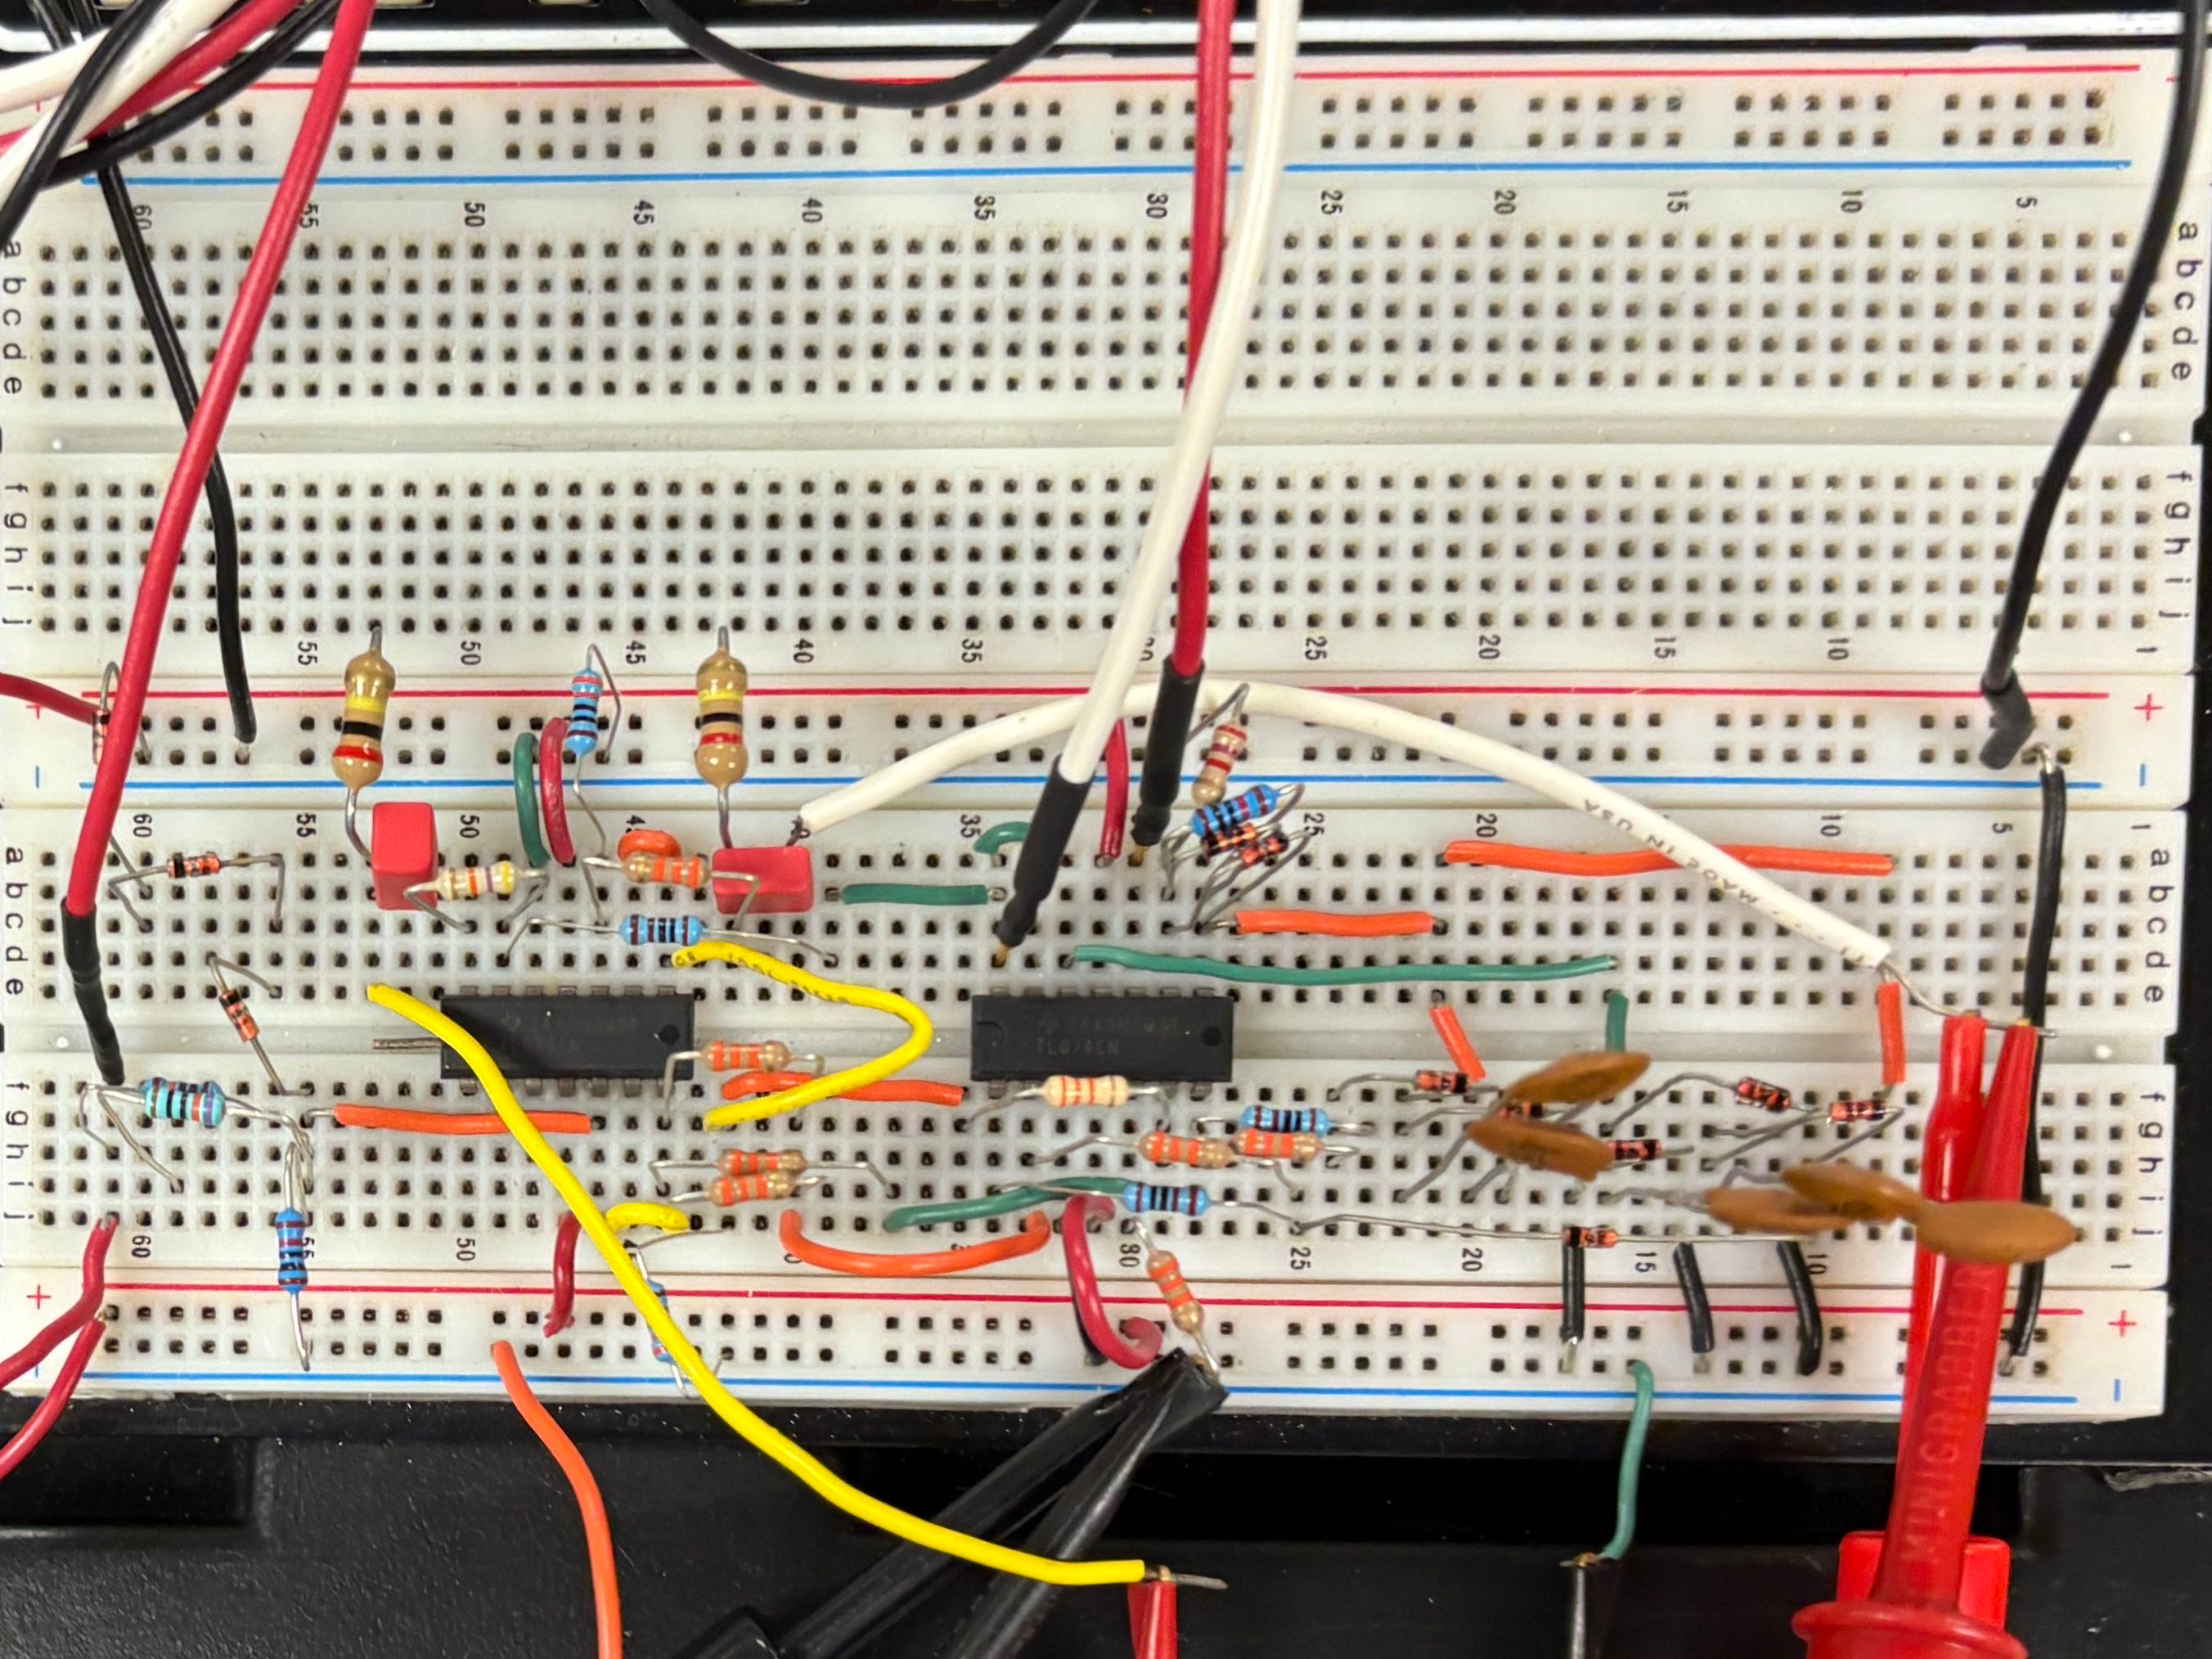
\includegraphics[width=0.8\textwidth]{../assets/breadboard.png}
    \caption{The circuit, implemented on breadboard. This may be modified to use the remaining op-amp on the bottom left to buffer the output for output to an amplifier.}
    \label{fig:breadboard}
    \par\noindent\rule{\textwidth}{0.4pt}
\end{figure}

\begin{figure}[H]
    \par\noindent\rule{\textwidth}{0.4pt}
    \centering
    
    % Create a 2x2 grid layout
    \begin{minipage}[t]{0.48\textwidth}
        % First column - subfigures (a) and (b)
        \begin{subfigure}{\textwidth}
            \vspace*{2em}
            \captionsetup{labelformat=empty}
            \begin{picture}(0,0)
                \put(-90,-10){\small\textbf{(a)}}
            \end{picture}
            \centering
            \resizebox{\textwidth}{!}{%
                \begin{circuitikz}
                    \tikzstyle{every node}=[font=\large]
                    \draw (8.25,14.25) node[op amp,scale=1, yscale=-1] (opamp2) {};
                    \draw (opamp2.+) to[short] (6.75,14.75);
                    \draw (opamp2.-) to[short] (6.75,13.75);
                    \draw (9.45,14.25) to[short](9.75,14.25);
                    \draw (0.75,14.25) to[C,l=$1\,\mu\text{F}$] (-1.25,14.25);
                    \draw (1.75,14.25) to[R,l=$33\,\text{k}\Omega$] (3.5,14.25);
                    \draw (6.75,13.75) to[short] (6.75,12.75);
                    \draw (6.75,12.75) to[short] (9.75,12.75);
                    \draw (9.75,12.75) to[short] (9.75,14.25);
                    \node at (4,14.25) [circ] {};
                    \draw (5.75,14.25) to[short] (5.75,14.75);
                    \draw (5.75,14.75) to[short] (6.75,14.75);
                    \draw (3.5,14.25) to[short] (4,14.25);
                    \draw (4,14.25) to[short] (5.75,14.25);
                    \draw (0.75,14.25) to[short] (1.75,14.25);
                    \node at (9.75,14.25) [circ] {};
                    \draw (-1.25,14.25) to[short, -o] (-2,14.25) node[above] {In};
                    \draw (0.75,14.25) to[R,l=$200\,\text{k}\Omega$] (0.75,11.75);
                    \draw (0.75,11.75) to (0.75,11.25) node[ground]{};
                    \draw (4,14.25) to[R,l=$330\,\text{k}\Omega$] (4,11.75);
                    \draw (4,11.75) to (4,11.25) node[ground]{};
                    \draw (8,6) node[op amp,scale=1, yscale=-1] (opamp2) {};
                    \draw (opamp2.+) to[short] (6.5,6.5);
                    \draw (opamp2.-) to[short] (6.5,5.5);
                    \draw (9.2,6) to[short](9.5,6);
                    \draw (1.5,6) to[R,l=$33\,\text{k}\Omega$] (3.25,6);
                    \draw (6.5,5.5) to[short] (6.5,4.5);
                    \draw (6.5,4.5) to[short] (9.5,4.5);
                    \draw (9.5,4.5) to[short] (9.5,6);
                    \node at (3.75,6) [circ] {};
                    \draw (5.5,6) to[short] (5.5,6.5);
                    \draw (5.5,6.5) to[short] (6.5,6.5);
                    \draw (3.25,6) to[short] (3.75,6);
                    \draw (3.75,6) to[short] (5.5,6);
                    \draw (0.5,6) to[short] (1.5,6);
                    \node at (9.5,6) [circ] {};
                    \draw (0.5,6) to[R,l=$10\,\text{k}\Omega$] (0.5,3.5);
                    \draw (0.5,3.5) to (0.5,3) node[ground]{};
                    \draw (3.75,6) to[D] (3.75,4);
                    \draw (3.75,4) to[D] (3.75,2);
                    \draw (3.75,2) to[D] (3.75,0);
                    \draw (3.75,0) to (5.75,0) node[ground]{};
                    \draw (0.5,6) to[R,l=$100\,\text{k}\Omega$] (-2.5,6);
                    \draw (0.5,8) to[R,l=$100\,\text{k}\Omega$] (-2.5,8);
                    \draw (0.5,6) to[short] (0.5,8);
                    \draw (-5.75,11.25) to[potentiometer] (-5.75,7.75);
                    \draw (-5.25,9.5) to[short] (-2.5,9.5);
                    \draw (-2.5,9.5) to[short] (-2.5,8);
                    \draw (-2.5,6) to[short] (-5.75,6);
                    \node [font=\large] at (-6.75,8) {-12V};
                    \node [font=\large] at (-6.75,11) {+12V};
                    \node [font=\large] at (-6,6.5) {+5.2V};
                    \draw (17.5,6) to[short] (17.5,6.5);
                    \draw (17.5,6) to[short] (18.5,6);
                    \draw (15.75,6) to[short] (17.5,6);
                    \draw (15.75,6) to[R,l=$33\,\text{k}\Omega$] (13.25,6);
                    \draw (13.25,6) to[short] (9.5,6);
                    \draw (20,5.5) node[op amp,scale=1] (opamp3) {};
                    \draw (opamp3.+) to[short] (18.5,5);
                    \draw (opamp3.-) to[short] (18.5,6);
                    \draw (21.2,5.5) to[short](21.5,5.5);
                    \draw (18.5,5) to (18.5,3.75) node[ground]{};
                    \draw (17.5,6.5) to[short] (17.5,7.25);
                    \draw (21.5,7.25) to[R,l=$2\,\text{k}\Omega$] (21.5,5.5);
                    \draw (18.25,7.75) to[R,l=$33\,\text{k}\Omega$] (20.5,7.75);
                    \draw (18.25,7.75) to[short] (17.5,7.75);
                    \draw (17.5,7.75) to[short] (17.5,7.25);
                    \draw (21.5,7.25) to[short] (21.5,7.75);
                    \draw (21.5,7.75) to[short] (20.5,7.75);
                    \draw (17.5,7.75) to[short] (15.5,7.75);
                    \draw (13.5,7.75) to[R,l=$33\,\text{k}\Omega$] (15.5,7.75);
                    \draw (13.5,7.75) to[short] (12.75,7.75);
                    \draw (12.75,7.75) to[short] (12.75,14.25);
                    \draw (19.25,13.75) node[op amp,scale=1] (opamp4) {};
                    \draw (opamp4.+) to[short] (17.75,13.25);
                    \draw (opamp4.-) to[short] (17.75,14.25);
                    \draw (20.45,13.75) to[short](20.75,13.75);
                    \draw (17.75,13.25) to[R,l=$33\,\text{k}\Omega$] (17.75,11.5);
                    \draw (15.75,13.25) to[R,l=$33\,\text{k}\Omega$] (17.75,13.25);
                    \draw (14.25,14.25) to[R,l=$33\,\text{k}\Omega$] (16.25,14.25);
                    \draw (16.25,14.25) to[short] (17.75,14.25);
                    \draw (15.75,13.25) to[short] (12.75,13.25);
                    \draw (10.75,6) to[short] (10.75,13.25);
                    \draw (10.75,13.25) to[short] (12.75,13.25);
                    \draw (9.75,14.25) to[short] (14.25,14.25);
                    \draw (17.75,11.5) to (17.75,10.5) node[ground]{};
                    \draw (20.75,13.75) to[R,l=$10\,\text{k}\Omega$] (20.75,15.5);
                    \draw (20.25,16) to[R,l=$10\,\text{k}\Omega$] (17.75,16);
                    \draw (17.75,16) to[short] (17.75,14.25);
                    \draw (20.25,16) to[short] (20.75,16);
                    \draw (20.75,16) to[short] (20.75,15.5);
                    \draw (20.75,16) to[short] (27.25,16);
                    \draw (21.5,7.75) to[short] (27.25,7.75);
                    \draw (27.25,15.5) to[D] (27.25,14.25);
                    \draw (27.25,14.25) to[D] (27.25,13);
                    \draw (27.25,13) to[D] (27.25,12);
                    \draw (27.25,12) to[D] (27.25,10.75);
                    \draw (27.25,10.75) to[D] (27.25,9.5);
                    \draw (27.25,9.5) to[D] (27.25,8.25);
                    \draw (27.25,7.75) to[short] (27.25,8.25);
                    \draw (27.25,15.5) to[short] (27.25,16);
                    \draw (27.25,14.25) to[C] (25,14.25);
                    \draw (27.25,13) to[C] (25,13);
                    \draw (27.25,12) to[C] (25,12);
                    \draw (27.25,10.75) to[C] (25,10.75);
                    \draw (27.25,9.5) to[C] (25,9.5);
                    \draw (25,10.75) to (24.75,10.75) node[ground]{};
                    \draw (25,12) to (24.75,12) node[ground]{};
                    \draw (25,13) to (24.75,13) node[ground]{};
                    \draw (25,14.25) to[short] (23.25,14.25);
                    \draw (23.25,14.25) to[short] (23.25,9.5);
                    \draw (23.25,9.5) to[short] (25,9.5);
                    \draw (27.25,12) to[short] (29.5,12);
                    \draw (31,11.5) node[op amp,scale=1, yscale=-1] (opamp5) {};
                    \draw (opamp5.+) to[short] (29.5,12);
                    \draw (opamp5.-) to[short] (29.5,11);
                    \draw (32.2,11.5) to[short](32.5,11.5);
                    \draw (29.5,11) to[short] (29.5,9.75);
                    \draw (29.5,9.75) to[short] (32.5,9.75);
                    \draw (32.5,11.5) to[short] (32.5,9.75);
                    \draw (32.5,11.5) to[R,l=$1\,\text{k}\Omega$] (34.5,11.5);
                    \draw (36,11) node[op amp,scale=1] (opamp6) {};
                    \draw (opamp6.+) to[short] (34.5,10.5);
                    \draw (opamp6.-) to[short] (34.5,11.5);
                    \draw (37.2,11) to[short](37.5,11);
                    \draw (34.5,10.5) to (33.75,10.5) node[ground]{};
                    \draw (34.5,11.5) to[short] (34.5,13);
                    \draw (35,13) to[R,l=$47\,\text{k}\Omega$] (37,13);
                    \draw (37,13) to[short] (37.5,13);
                    \draw (37.5,13) to[short] (37.5,11);
                    \draw (35,13) to[short] (34.5,13);
                    \draw (37.5,11) to[C,l=$1\,\mu\text{F}$] (39.5,11);
                    \draw (39.5,11) to[R,l=$200\,\text{k}\Omega$] (39.5,8.5);
                    \draw (39.5,8.5) to (39.5,8) node[ground]{};
                    \draw (23.25,14.25) to[short] (23.25,18.5);
                    \draw (27,18.5) node[op amp,scale=1, xscale=-1] (opamp7) {};
                    \draw (opamp7.+) to[short] (28.5,18);
                    \draw (opamp7.-) to[short] (28.5,19);
                    \draw (25.8,18.5) to[short](25.5,18.5);
                    \draw (28.5,19) to[short] (28.5,20.5);
                    \draw (25.5,18.5) to[short] (25.5,20.5);
                    \draw (25.5,20.5) to[R,l=$10\,\text{k}\Omega$] (28.5,20.5);
                    \draw (28.5,21.75) to[D] (25.5,21.75);
                    \draw (25.5,20.5) to[short] (25.5,21.75);
                    \draw (28.5,20.5) to[short] (28.5,23.25);
                    \draw (25.5,21.75) to[short] (25.5,23.25);
                    \draw (25.5,23.25) to[D] (28.5,23.25);
                    \draw (28.5,23.25) to[R,l=$2.7\,\text{k}\Omega$] (28.5,25.75);
                    \draw (28.5,25.75) to (29.75,25.75) node[ground]{};
                    \draw (25.5,18.5) to[short] (23.25,18.5);
                    \draw (29.5,16.75) to[potentiometer] (29.5,19.25);
                    \draw (29.5,17) to[short] (29.5,12);
                    \draw (29,18) to[short] (28.5,18);
                    \draw (29.5,19.25) to (30.75,19.25) node[ground]{};
                    \draw (39.5,11) to[short, -o] (43.25,11) node[right] {Out};
                    \node at (39.5,11) [circ] {};
                    \node at (37.5,11) [circ] {};
                    \node at (34.5,11.5) [circ] {};
                    \node at (32.5,11.5) [circ] {};
                    \node at (29.5,12) [circ] {};
                    \node at (25.5,18.5) [circ] {};
                    \node at (25.5,20.5) [circ] {};
                    \node at (25.5,21.75) [circ] {};
                    \node at (28.5,21.75) [circ] {};
                    \node at (28.5,20.5) [circ] {};
                    \node at (28.5,23.25) [circ] {};
                    \node at (27.25,9.5) [circ] {};
                    \node at (27.25,10.75) [circ] {};
                    \node at (27.25,12) [circ] {};
                    \node at (27.25,13) [circ] {};
                    \node at (27.25,14.25) [circ] {};
                    \node at (21.5,7.75) [circ] {};
                    \node at (17.5,7.75) [circ] {};
                    \node at (17.5,6) [circ] {};
                    \node at (17.75,13.25) [circ] {};
                    \node at (20.75,16) [circ] {};
                    \node at (17.75,14.25) [circ] {};
                    \node at (12.75,14.25) [circ] {};
                    \node at (10.75,6) [circ] {};
                    \node at (0.5,6) [circ] {};
                \end{circuitikz}
            }
            \label{fig:circuit}
        \end{subfigure}
        
        \vspace{2em}
        
        \begin{subfigure}{\textwidth}
            \captionsetup{labelformat=empty}
            \begin{picture}(0,0)
                \put(-90,15){\small\textbf{(b)}}
            \end{picture}
            \centering
            \includegraphics[width=\textwidth]{../../code/filter_output.pdf}
            \label{fig:output}
        \end{subfigure}
    \end{minipage}
    \hfill
    \begin{minipage}[t]{0.48\textwidth}
        % Second column - subfigures (c) and (d)
        \begin{subfigure}{\textwidth}
            \captionsetup{labelformat=empty}
            \begin{picture}(0,0)
                \put(-110,-20){\small\textbf{(c)}}
            \end{picture}
            \centering
            \includegraphics[width=\textwidth]{../../code/bode_plot.pdf}
            \label{fig:bode}
        \end{subfigure}
        
        \vspace{2em}
        
        \begin{subfigure}{\textwidth}
            \captionsetup{labelformat=empty}
            \begin{picture}(0,0)
                \put(-90,15){\small\textbf{(d)}}
            \end{picture}
            \centering
            \includegraphics[width=\textwidth]{../../code/voltage_sweep.pdf}
            \label{fig:voltage-sweep}
        \end{subfigure}
    \end{minipage}
    
    \caption{\textbf{(a)} The completed circuit schematic, combining all previous parts. \textbf{(b)} The input signal (red) versus the output signal with moderate resonance and cutoff (blue). \textbf{(c)} Bode plot showing the bode frequency response of the circuit. This circuit is a low-pass filter which operates well within the human range of hearing. The 3 dB point for this circuit is also located at 12.65 kHz, and is accompianied by a decaying output until the MHz regime. The phase is an incomplete descriptor of the circuit, as resonance acts as a third parameter which results in unusual phenomena. This does, however, provide insight into the behavior of resonance as a function of frequency. The input signal is dominated by resonance at the $<10^2$ Hz regime, producing a sinusoidal wave. This vanishes between the $10^2-10^4$ Hz regime, where we see ideal operation at the parameters set, similar to (b). After this point, the signal again is overtaken by resonance. The sharp transition at $10^5$ Hz is likely associated with a final unique phase of the circuit, as the frequency is so massive that the waveform becomes approximately flat as the negative feedback the circuit operates on is no longer able to keep up with the input signal. \textbf{(d)} Voltage sweep analysis showing the circuit's response to varying input voltages. Due to the amplification stages of the circuit, resonance intensity is proportional to input voltage, shown in the legend. Furthermore, resonance is clearly defined at all but the smallest (millivolt) input voltages due to noise overtaking the signal.}
    \label{fig:circuit-combined}
    
    \par\noindent\rule{\textwidth}{0.4pt}
\end{figure}


\bibliographystyle{plain}  % or another style like 'alpha', 'unsrt', etc.
\bibliography{./_citations.bib}
